\subsection{Версия 2: поиск высокотемпературной материальной архитектуры}

Вторая версия расчетного пайплайна отвечает уже не на вопрос о штатной циркониевой оболочке, а на вопрос о том, какой класс материалов нужен для реакторной схемы, способной подвести энергию к тонкой паровой области и открыть путь к ненулевому выходу \(H_2\). Входами остаются геометрия одного метра твэла, давление \(15.5\,\mathrm{МПа}\), толщина паровой прослойки и импульс \(E_{\mathrm{вв}}\). Основные выходы не меняются: \(T_s^{\max}\), запас топлива и оболочки до пределов и верхняя энергетическая оценка \(H_2\).

Эта версия не заменяет химико-механическую квалификацию материалов. \(ZrC\)-центричная ветка введена как более правдоподобное исследовательское направление после отсева \(UO_2\), \(UN\), \(UC\), Zircaloy, Mo и SiC/SiC. \(HfC\)--W оставлен как оптимистический тепловой контрфакт: он показывает, что математическое тепловое окно может открыться, но не является предложением материала из-за гафния и парового окисления вольфрама \cite{UshakovCarbides2019,PetersonZrC2023,SabourinTungstenSteam2011}.

\begin{figure}[H]
    \centering
    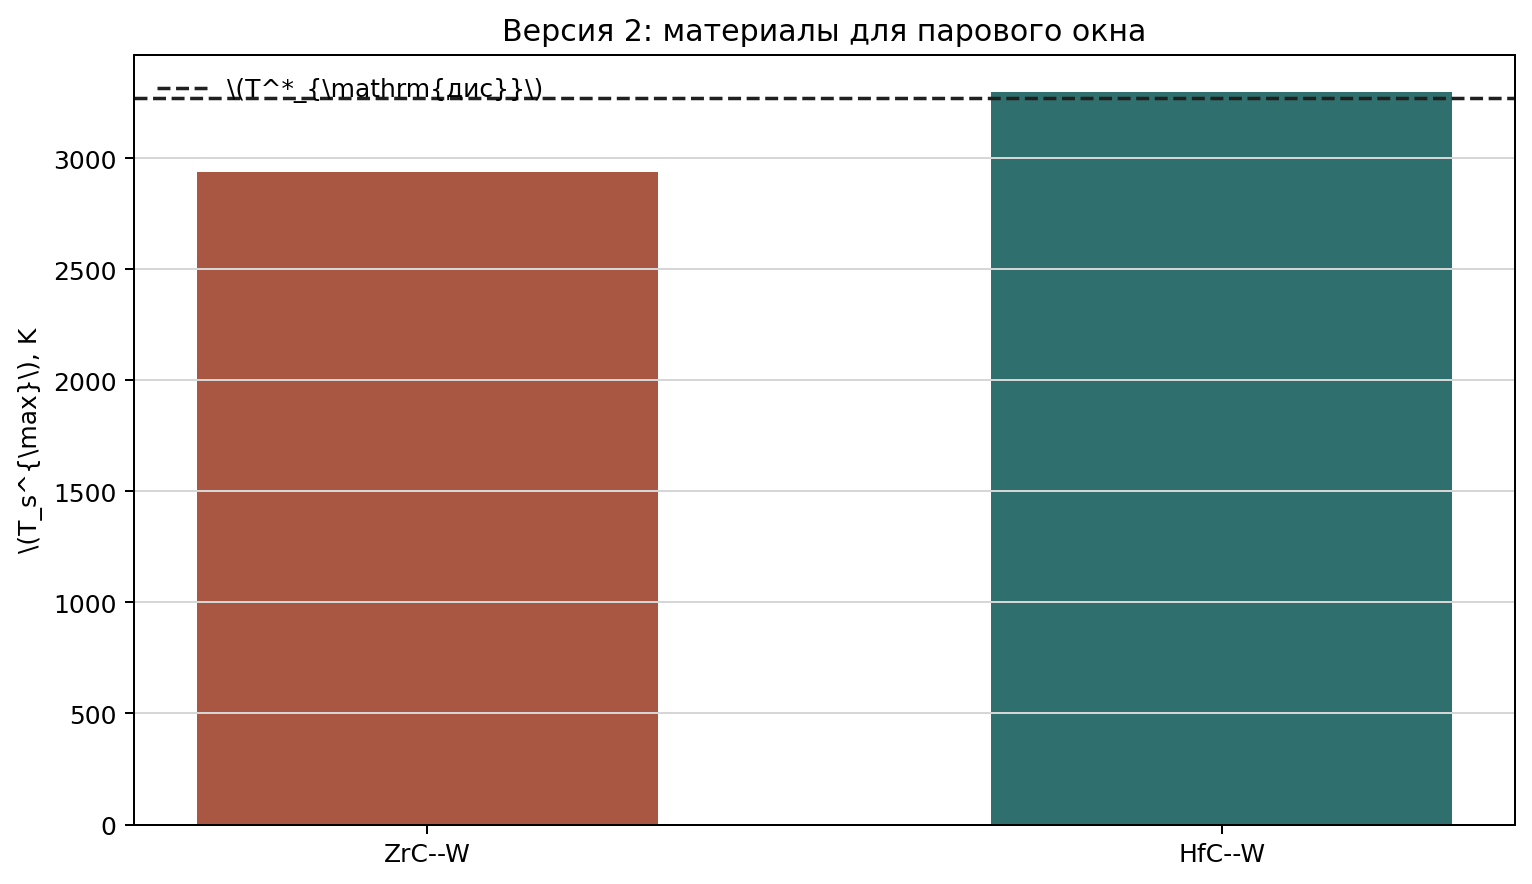
\includegraphics[width=0.90\textwidth]{figures/pipeline_v2_material_window.png}
    \caption{Версия 2 пайплайна: сравнение высокотемпературных материаловедческих суррогатов по максимуму температуры паровой прослойки. Положительный тепловой признак не означает химически квалифицированную оболочку.}
    \label{fig:pipelineV2MaterialWindow}
\end{figure}

\begin{table}[H]
    \centering
    \caption{Версия 2 пайплайна: отборочные сценарии для новой материальной структуры.}
    \label{tab:pipelineV2MaterialScenarios}
    \footnotesize
    \resizebox{\textwidth}{!}{%
    \begin{tabular}{@{}p{4.0cm}rp{2.0cm}p{2.2cm}p{3.0cm}p{6.0cm}@{}}
    \hline
    Сценарий & \(E_{\mathrm{вв}}\), кДж/м & \(T_s^{\max}\), K & Окно до пределов & Класс результата & Роль в дипломе \\
    \hline
    \(ZrC\)--W, исследовательский суррогат & 520 & 2938 & нет & материалы целы, окно ниже порога & более правдоподобная ZrC-центричная ветка; наружный W не квалифицирован по пару \\
\(HfC\)--W, тепловой верхний контрфакт & 480 & 3301 & да & тепловое окно достигнуто & оптимистический тепловой предел; материал не квалифицирован по нейтронике и пару \\
    \hline
    \end{tabular}
    }
\end{table}

Инженерная трактовка второй версии такая: цель диплома остается положительной -- найти расчетную область, где реакторная система может получить высокотемпературный пар и ненулевую верхнюю оценку \(H_2\). Но путь к этой области проходит через последовательный отбор: сначала исключается штатная циркониевая оболочка, затем строится тепловой контрфакт, и только после этого можно ставить отдельную задачу о ZrC-центричном материале, паровой химии, механике и нейтронной совместимости.
